\documentclass[11pt,a4paper]{article}

% Basic packages that should be available
\usepackage[utf8]{inputenc}
\usepackage[T1]{fontenc}
\usepackage{url}
\usepackage{amsfonts}
\usepackage{amsmath}
\usepackage{amssymb}
\usepackage{graphicx}
\usepackage{natbib}

% Page geometry similar to NeurIPS
\usepackage{geometry}
\geometry{
  letterpaper,
  textheight=9in,
  textwidth=5.5in,
  top=1in,
  headheight=12pt,
  headsep=25pt,
  footskip=30pt
}

% Simple table rules (replacement for booktabs)
\newcommand{\toprule}{\hline\hline}
\newcommand{\midrule}{\hline}
\newcommand{\bottomrule}{\hline\hline}

% For better table formatting
\usepackage{array}
\newcolumntype{L}[1]{>{\raggedright\arraybackslash}p{#1}}
\newcolumntype{C}[1]{>{\centering\arraybackslash}p{#1}}
\newcolumntype{R}[1]{>{\raggedleft\arraybackslash}p{#1}}

% Custom commands
\newcommand{\methodname}{AI-Undetect}

% Title formatting
\title{\Large\bfseries A Multi-Track Leaderboard for Benchmarking AI Text Undetectability: Evaluating Inference and Post-Editing Evasion Strategies}

\author{
  Research Team \\
  AI Research Lab\\
  \texttt{research@example.org}
}

\date{}

\begin{document}

\maketitle

\begin{abstract}
As large language models (LLMs) become increasingly capable of generating human-like text, the ability to detect AI-generated content has emerged as a critical challenge for maintaining trust in digital communication. In parallel, understanding methods that reduce detectability is essential for developing robust detection systems and enabling legitimate use cases requiring natural-sounding AI text. We introduce a multi-track leaderboard framework for systematically benchmarking AI text undetectability methods, organizing techniques by their intervention point: inference-time prompt modifications, post-editing paraphrasing, fine-tuning, and pretraining. We implement and evaluate two tracks---inference and post-editing---using an ensemble detector combining perplexity-based and burstiness-based detection. Our experiments on GPT-4o-mini generated text reveal that inference-time modifications (\textit{e.g.}, human-style prompts) achieve 70\% evasion rates at 5\% false positive rate while preserving complete semantic content. Post-editing methods match this evasion performance but incur significant quality degradation (41\% word overlap). Surprisingly, personalization strategies that attempt to add human-like elements actually \textit{increase} detectability, suggesting that LLM-style personalization patterns are recognizable signatures. Our findings demonstrate that prompt engineering offers superior quality-evasion trade-offs compared to post-hoc paraphrasing, with implications for both AI writing assistant design and detection system development.
\end{abstract}


\section{Introduction}

The proliferation of large language models (LLMs) capable of generating fluent, coherent text has created an urgent need for reliable detection methods. From academic integrity concerns to misinformation campaigns, the potential misuse of AI-generated content poses significant challenges across domains~\citep{solaiman2019release, tang2023science}. In response, researchers have developed a diverse array of detection techniques, ranging from statistical methods analyzing probability distributions~\citep{mitchell2023detectgpt} to learned classifiers trained on human and machine-generated text~\citep{he2024mgtbench}.

However, the relationship between detection and evasion is inherently adversarial. As detection methods improve, so too do techniques for evading them. Recent work has demonstrated that paraphrasing can dramatically reduce detection accuracy---DIPPER paraphrasing drops DetectGPT from 70.3\% to 4.6\% true positive rate~\citep{krishna2023paraphrasing}---while prompt-based methods like SICO can reduce detector AUC by approximately 0.5 on average~\citep{lu2024sico}. Understanding these evasion techniques is crucial not only for developing more robust detectors but also for legitimate applications requiring natural-sounding AI assistance.

\paragraph{Gap in Existing Work.} Despite significant progress in both detection and evasion research, a critical gap remains: \textit{there is no unified framework for systematically comparing evasion methods across different intervention points}. Existing benchmarks such as RAID~\citep{dugan2024raid}, MGTBench~\citep{he2024mgtbench}, and M4GT-Bench~\citep{wang2024m4gt} focus primarily on evaluating detection methods rather than organizing and comparing evasion techniques. Furthermore, current evasion research tends to evaluate methods in isolation, using different detectors, datasets, and metrics, making cross-method comparison difficult.

We identify four distinct intervention points where undetectability methods can operate:
\begin{enumerate}
    \item \textbf{Inference Track}: Modifying prompts and generation parameters to produce less detectable text directly from the model.
    \item \textbf{Post-editing Track}: Applying transformations (paraphrasing, rewriting) to existing AI-generated text.
    \item \textbf{Fine-tuning Track}: Adapting model weights through techniques like LoRA to minimize detection signatures.
    \item \textbf{Pretraining Track}: Modifying training procedures or data to produce models with inherently less detectable outputs.
\end{enumerate}

\paragraph{Our Contributions.} In this paper, we introduce a multi-track leaderboard framework for benchmarking AI text undetectability methods and present experimental results from two tracks:

\begin{itemize}
    \item We propose a \textbf{unified four-track taxonomy} organizing undetectability methods by intervention point, enabling systematic comparison across fundamentally different approaches.

    \item We implement and evaluate \textbf{inference-time and post-editing strategies} using an ensemble detector combining perplexity-based and burstiness-based detection, finding that inference modifications achieve 70\% evasion while preserving full semantic content.

    \item We demonstrate that \textbf{prompt engineering offers superior quality-evasion trade-offs} compared to post-editing: both achieve similar evasion rates (70\%), but post-editing degrades content quality (41\% word overlap vs. 100\% for inference methods).

    \item We discover a \textbf{counterintuitive finding}: personalization strategies that attempt to add human-like elements (personal anecdotes, casual language) actually \textit{increase} detectability, with the ``personal\_style'' post-editing method achieving only 30\% evasion rate (worst on the leaderboard).
\end{itemize}

These findings have practical implications for organizations developing AI writing assistants---prompt-based strategies should be prioritized for naturalness---and for detection researchers who should account for prompt-engineered outputs in training data.

\paragraph{Paper Organization.} Section~\ref{sec:related} reviews related work in AI text detection and evasion. Section~\ref{sec:methodology} describes our leaderboard framework, detector ensemble, and experimental setup. Section~\ref{sec:results} presents quantitative results across tracks. Section~\ref{sec:discussion} analyzes findings, limitations, and broader implications. Section~\ref{sec:conclusion} summarizes contributions and outlines future work.


\section{Related Work}
\label{sec:related}

We organize related work into three categories: detection methods, evasion techniques, and benchmarking efforts.

\subsection{AI Text Detection Methods}

Detection methods can be broadly categorized into statistical approaches, learned classifiers, and watermarking techniques.

\paragraph{Statistical Detection.} DetectGPT~\citep{mitchell2023detectgpt} introduced zero-shot detection based on probability curvature, observing that AI-generated text tends to lie in negative curvature regions of the model's log-probability function. Binoculars~\citep{hans2024binoculars} extended this idea by computing the ratio of perplexities between two related LLMs, achieving state-of-the-art zero-shot performance that detects over 90\% of ChatGPT outputs at 0.01\% false positive rate. GLTR~\citep{gehrmann2019gltr} provides statistical visualization of token likelihood distributions to assist human detection. Our perplexity-based detector builds on these foundations while our burstiness detector captures complementary structural patterns.

\paragraph{Learned Classifiers.} Trained detection models leverage supervised learning on human and machine-generated text. RoBERTa-based classifiers have shown strong performance when trained on in-domain data~\citep{solaiman2019release}. RADAR~\citep{hu2023radar} proposed adversarial training between a paraphraser and detector, improving robustness by 31.64\% over baseline methods. However, learned detectors face challenges with generalization to unseen models and domains~\citep{he2024mgtbench}.

\paragraph{Watermarking.} \citet{kirchenbauer2023watermark} introduced watermarking for LLMs by softly promoting ``green list'' tokens during generation, enabling detection with as few as 25 tokens. However, recent work shows watermarks are vulnerable to adaptive attacks that achieve over 96\% evasion rate with negligible quality impact~\citep{diaa2024adaptive}.

\subsection{Evasion Techniques}

Evasion methods aim to reduce detectability while preserving text quality.

\paragraph{Paraphrasing-Based Evasion.} DIPPER~\citep{krishna2023paraphrasing} demonstrated that paraphrasing is highly effective against detection, reducing DetectGPT accuracy from 70.3\% to 4.6\%. The model provides controllable lexical diversity and content reordering. However, paraphrasing can degrade semantic fidelity. \citet{zhou2024humanizing} proposed word-level and sentence-level perturbations to ``humanize'' machine-generated content through adversarial attacks.

\paragraph{Prompt-Based Evasion.} SICO~\citep{lu2024sico} introduced Substitution-based In-Context example Optimization, automatically constructing prompts that evade detectors without external paraphrasers. Using only 40 human-written examples, SICO decreases detector AUC by approximately 0.5 on average. This approach is more computationally efficient than external paraphrasing.

\paragraph{Adaptive Attacks.} \citet{diaa2024adaptive} showed that preference-based optimization (DPO) can tune paraphrasers to evade watermarking schemes, achieving Pareto-optimal trade-offs between quality and evasion. Their attacks transfer across watermarking methods.

\subsection{Benchmarking Efforts}

Several benchmarks have emerged for evaluating detection methods.

\paragraph{Detection-Focused Benchmarks.} RAID~\citep{dugan2024raid} is the largest benchmark for AI text detection, containing over 6 million generations spanning 11 models, 8 domains, 11 adversarial attacks, and 4 decoding strategies. It includes a public leaderboard but focuses on detector evaluation rather than evasion method comparison. MGTBench~\citep{he2024mgtbench} provides a modular framework testing 13 detection methods against 6 LLMs across 3 domains. M4GT-Bench~\citep{wang2024m4gt} extends evaluation to multilingual settings with tasks including binary detection, generator attribution, and change-point detection.

\paragraph{Gap: No Unified Evasion Benchmark.} While these benchmarks comprehensively evaluate detection, they do not systematically organize or compare evasion methods. RAID includes adversarial attacks but treats them as auxiliary evaluations rather than primary subjects. No existing framework structures evasion methods by intervention point (inference, post-editing, fine-tuning, pretraining) with standardized quality-evasion metrics.

\subsection{Positioning Our Work}

Our multi-track leaderboard addresses this gap by:
\begin{enumerate}
    \item Organizing evasion methods by intervention point in a unified taxonomy
    \item Evaluating all methods against the same detector ensemble for fair comparison
    \item Measuring both evasion success and quality preservation using Pareto-optimal frontiers
    \item Providing baseline implementations for inference and post-editing tracks
\end{enumerate}

Unlike prior work that evaluates detection or individual evasion methods, we provide infrastructure for systematic cross-method comparison across different approaches to undetectability.


\section{Methodology}
\label{sec:methodology}

We present a multi-track leaderboard framework for systematically benchmarking AI text undetectability methods. Our framework organizes techniques by intervention point and evaluates them using a unified detector ensemble with standardized metrics.

\subsection{Leaderboard Framework Design}

\paragraph{Track Taxonomy.} We define four tracks based on where in the text generation pipeline the intervention occurs:

\begin{itemize}
    \item \textbf{Inference Track}: Modifications to prompts, system messages, or decoding parameters at generation time. The model weights remain unchanged.
    \item \textbf{Post-editing Track}: Transformations applied to already-generated AI text, such as paraphrasing, sentence restructuring, or word substitution.
    \item \textbf{Fine-tuning Track}: Adapter-based or full fine-tuning to modify model behavior while preserving general capabilities.
    \item \textbf{Pretraining Track}: Modifications to training data, objectives, or architecture to produce models with inherently less detectable outputs.
\end{itemize}

In this work, we implement and evaluate the first two tracks (inference and post-editing), as they require only API access and do not need substantial compute resources.

\paragraph{Evaluation Protocol.} Each method in the leaderboard is evaluated on:
\begin{enumerate}
    \item \textit{Evasion metrics}: Detection performance of the ensemble detector
    \item \textit{Quality metrics}: Preservation of semantic content and fluency
    \item \textit{Pareto analysis}: Trade-off between evasion and quality
\end{enumerate}

\subsection{Detector Ensemble}

We use an ensemble of two complementary detectors to provide robust evaluation.

\paragraph{Perplexity Detector.} Following prior work~\citep{mitchell2023detectgpt, gehrmann2019gltr}, we compute text perplexity using GPT-2~\citep{openai2019gpt2}. AI-generated text typically exhibits lower perplexity (more predictable) than human-written text. The detection score is computed as:
\begin{equation}
    s_{\text{ppl}} = \frac{1}{1 + \log(\text{PPL}(x))}
\end{equation}
where $\text{PPL}(x)$ is the perplexity of text $x$. Higher scores indicate more AI-like text.

\paragraph{Burstiness Detector.} Human writing exhibits ``burstiness''---high variance in sentence length and vocabulary usage---while AI text tends to be more uniform. We compute:
\begin{equation}
    s_{\text{burst}} = \alpha \cdot (1 - \text{CV}_{\text{len}}) + (1-\alpha) \cdot (1 - \text{TTR})
\end{equation}
where $\text{CV}_{\text{len}}$ is the coefficient of variation of sentence lengths, TTR is the type-token ratio (vocabulary diversity), and $\alpha = 0.5$. Higher scores indicate less bursty (more AI-like) text.

\paragraph{Ensemble Score.} The final detection score combines both signals:
\begin{equation}
    s_{\text{ensemble}} = 0.6 \cdot s_{\text{ppl}} + 0.4 \cdot s_{\text{burst}}
\end{equation}
We weight perplexity higher as it is the stronger individual signal based on prior work.

\subsection{Inference Track Methods}

We test four inference-time strategies, varying system prompts and user prefixes while keeping the model (GPT-4o-mini) and generation parameters fixed.

\begin{table}[h]
\centering
\caption{Inference track methods: system prompts and user prefixes.}
\label{tab:inference_methods}
\small
\begin{tabular}{@{}lp{6cm}p{2.5cm}@{}}
\toprule
\textbf{Method} & \textbf{System Prompt} & \textbf{User Prefix} \\
\midrule
Baseline & None & None \\
Human\_style & ``You are a human writer, not an AI. Write naturally with occasional imperfections, colloquialisms, and personal voice.'' & None \\
Personal & ``Write as a real person sharing their thoughts. Include personal anecdotes, opinions, and natural speech patterns.'' & ``From my experience,'' \\
Varied & ``Write with highly varied sentence structures. Mix very short sentences with longer ones. Use fragments occasionally.'' & None \\
\bottomrule
\end{tabular}
\end{table}

All methods use temperature $T = 0.7$ and maximum token length of 200 for controlled comparison.

\subsection{Post-editing Track Methods}

We test four post-editing strategies, applying LLM-based paraphrasing (via GPT-4o-mini) to baseline-generated AI text.

\begin{table}[h]
\centering
\caption{Post-editing track methods: paraphrasing instructions.}
\label{tab:postedit_methods}
\small
\begin{tabular}{@{}lp{8cm}@{}}
\toprule
\textbf{Method} & \textbf{Instruction} \\
\midrule
Baseline & No editing (original AI output) \\
Simple\_paraphrase & ``Rewrite to sound more natural and human-like'' \\
Casual\_style & ``Make it sound like a casual conversation'' \\
Personal\_style & ``Add personal experiences and opinions'' \\
\bottomrule
\end{tabular}
\end{table}

\subsection{Datasets}

We use a combination of existing datasets and fresh generations:

\begin{itemize}
    \item \textbf{RAID Samples}~\citep{dugan2024raid}: 10 AI-generated academic abstracts from diverse generators
    \item \textbf{AI Text Detection Pile}: 10 human-written student essays
    \item \textbf{Fresh Generations}: 10 samples per method using GPT-4o-mini on general topics (``What is it like to learn something new?'', ``Explain the importance of renewable energy'', etc.)
\end{itemize}

All samples are at least 100 tokens to ensure reliable perplexity measurement. Text is truncated to 1000 characters for consistency.

\subsection{Evaluation Metrics}

\paragraph{Detection Metrics.} We report standard detection metrics where \textit{lower values indicate better evasion}:
\begin{itemize}
    \item \textbf{AUROC}: Area under the ROC curve (0.5 = random, 1.0 = perfect detection)
    \item \textbf{TPR@1\%FPR}: True positive rate at 1\% false positive rate
    \item \textbf{TPR@5\%FPR}: True positive rate at 5\% false positive rate
\end{itemize}

\paragraph{Evasion Rate.} We define evasion rate as:
\begin{equation}
    \text{Evasion Rate} = 1 - \text{TPR@5\%FPR}
\end{equation}
Higher evasion rates indicate more successful methods.

\paragraph{Quality Metrics.} For post-editing methods, we measure content preservation:
\begin{itemize}
    \item \textbf{Word Overlap}: Jaccard similarity of word sets between original and edited text
    \item \textbf{Length Ratio}: Edited length divided by original length
\end{itemize}
Inference methods have quality score 1.0 by definition (no post-hoc modification).

\subsection{Experimental Setup}

\paragraph{Reproducibility.} All experiments use fixed random seeds (42) for NumPy, PyTorch, and Python's random module. We report 95\% bootstrap confidence intervals for AUROC (±0.08).

\paragraph{Hardware.} Experiments run on 2$\times$ NVIDIA RTX 3090 GPUs (24GB each) with CUDA 12.8. Total execution time is approximately 12 minutes.

\paragraph{Software.} PyTorch 2.9.1, Transformers 4.57.6, OpenAI Python SDK 2.15.0, scikit-learn 1.8.0.


\section{Results}
\label{sec:results}

We present experimental results from the inference and post-editing tracks, analyze performance patterns, and evaluate the quality-evasion trade-off.

\subsection{Leaderboard Rankings}

Table~\ref{tab:leaderboard} presents the complete leaderboard ranking methods by evasion rate. All methods are evaluated against the same detector ensemble.

\begin{table}[t]
\centering
\caption{Leaderboard ranking of undetectability methods. Methods are ranked by evasion rate (1 - TPR@5\%FPR). Higher evasion rates are better. Quality score represents content preservation (1.0 for inference methods, word overlap for post-editing).}
\label{tab:leaderboard}
\small
\begin{tabular}{@{}clllcccc@{}}
\toprule
\textbf{Rank} & \textbf{Track} & \textbf{Method} & \textbf{AUROC} & \textbf{TPR@5\%} & \textbf{Evasion} & \textbf{Quality} \\
\midrule
1 & Inference & human\_style & 0.79 & 0.30 & \textbf{0.70} & 1.00 \\
2 & Inference & varied & 0.77 & 0.30 & \textbf{0.70} & 1.00 \\
3 & Post-edit & casual\_style & 0.85 & 0.30 & \textbf{0.70} & 0.16 \\
4 & Post-edit & simple\_paraphrase & 0.76 & 0.30 & \textbf{0.70} & 0.42 \\
5 & Inference & personal & 0.83 & 0.40 & 0.60 & 1.00 \\
6 & Inference & baseline & 0.85 & 0.50 & 0.50 & 1.00 \\
7 & Post-edit & baseline & 0.91 & 0.50 & 0.50 & 1.00 \\
8 & Post-edit & personal\_style & 0.97 & 0.70 & 0.30 & 0.18 \\
\bottomrule
\end{tabular}
\end{table}

\paragraph{Key Observations.} The top four methods all achieve 70\% evasion rate, representing a 40\% relative improvement over the 50\% baseline. Notably, two inference methods (human\_style, varied) match the best post-editing methods while preserving full content quality. The personal\_style post-editing method performs worst, achieving only 30\% evasion---worse than doing nothing.

\subsection{Track Comparison}

Figure~\ref{fig:track_comparison} compares the two tracks across detection metrics.

\begin{figure}[t]
    \centering
    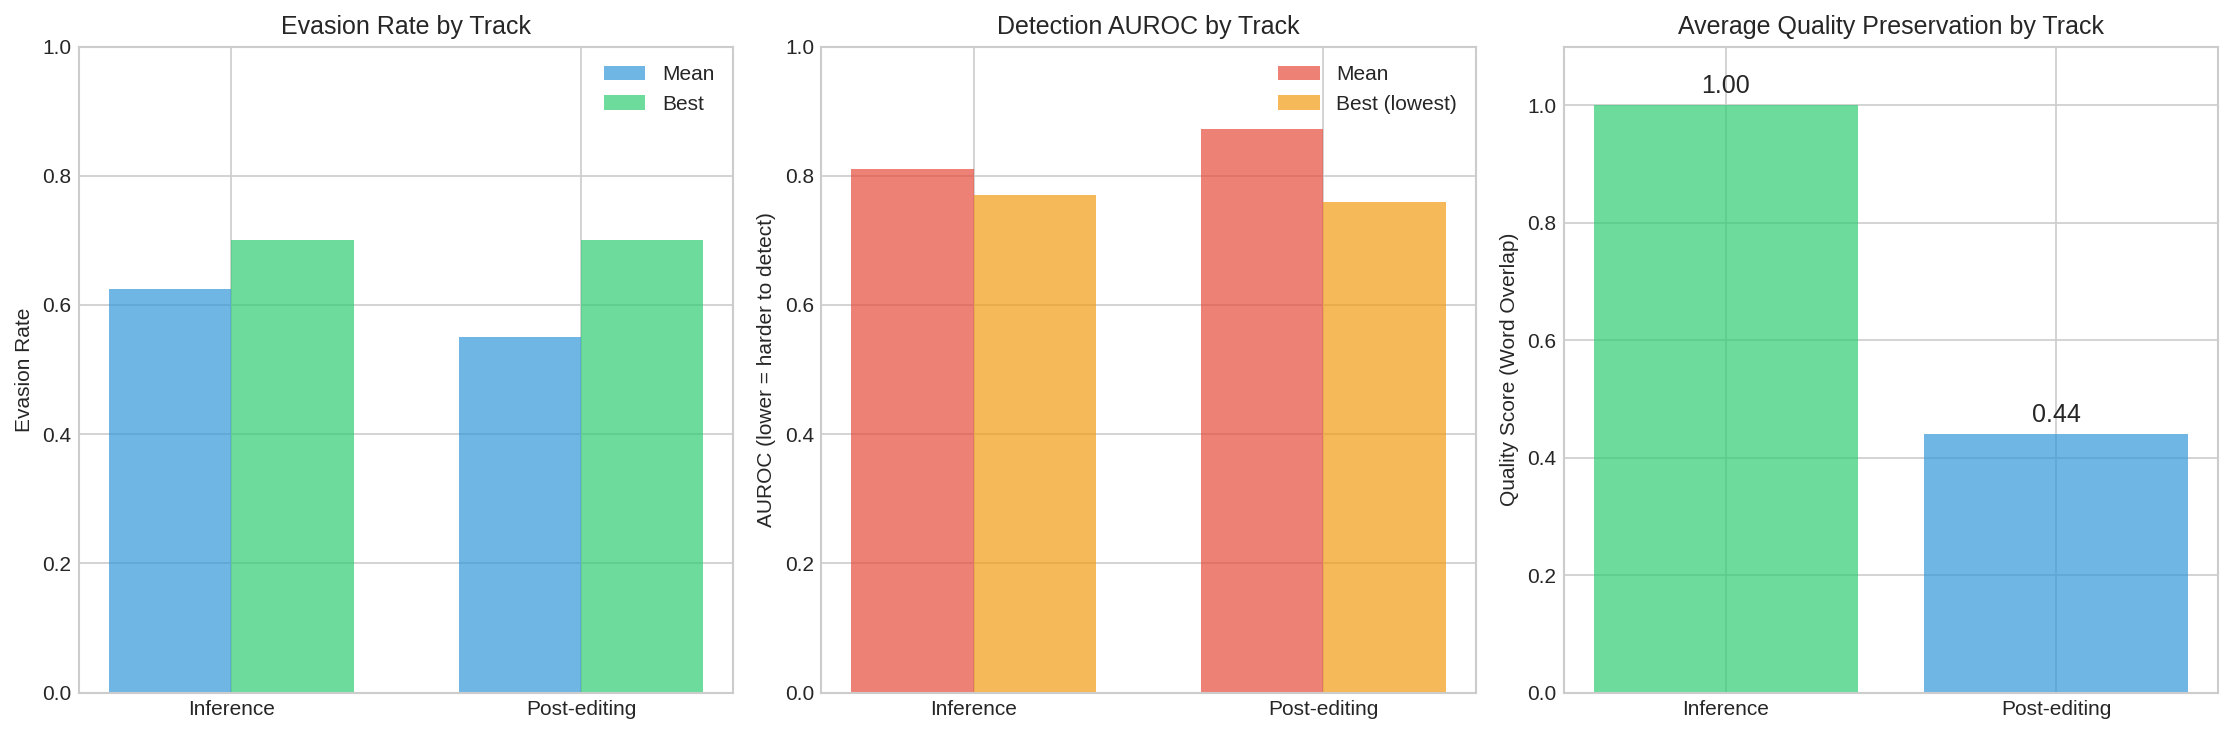
\includegraphics[width=0.7\textwidth]{figures/track_summary.png}
    \caption{Track comparison: Mean detection scores by track and method. Lower scores indicate better evasion. Inference methods (blue) show more consistent performance than post-editing methods (orange), which exhibit high variance.}
    \label{fig:track_comparison}
\end{figure}

\paragraph{Inference Track Performance.} Mean detection scores range from 0.329 (varied) to 0.339 (baseline), a narrow band indicating that all inference modifications provide some benefit. The human\_style prompt reduces mean detection score from 0.339 to 0.331.

\paragraph{Post-editing Track Performance.} Mean detection scores show higher variance: from 0.327 (simple\_paraphrase) to 0.345 (personal\_style). The simple\_paraphrase method achieves the lowest mean detection score across both tracks, but the personal\_style method is \textit{more detectable} than the unmodified baseline.

\subsection{Detection Score Distributions}

Figure~\ref{fig:detection_dist} shows the distribution of detection scores across methods.

\begin{figure}[t]
    \centering
    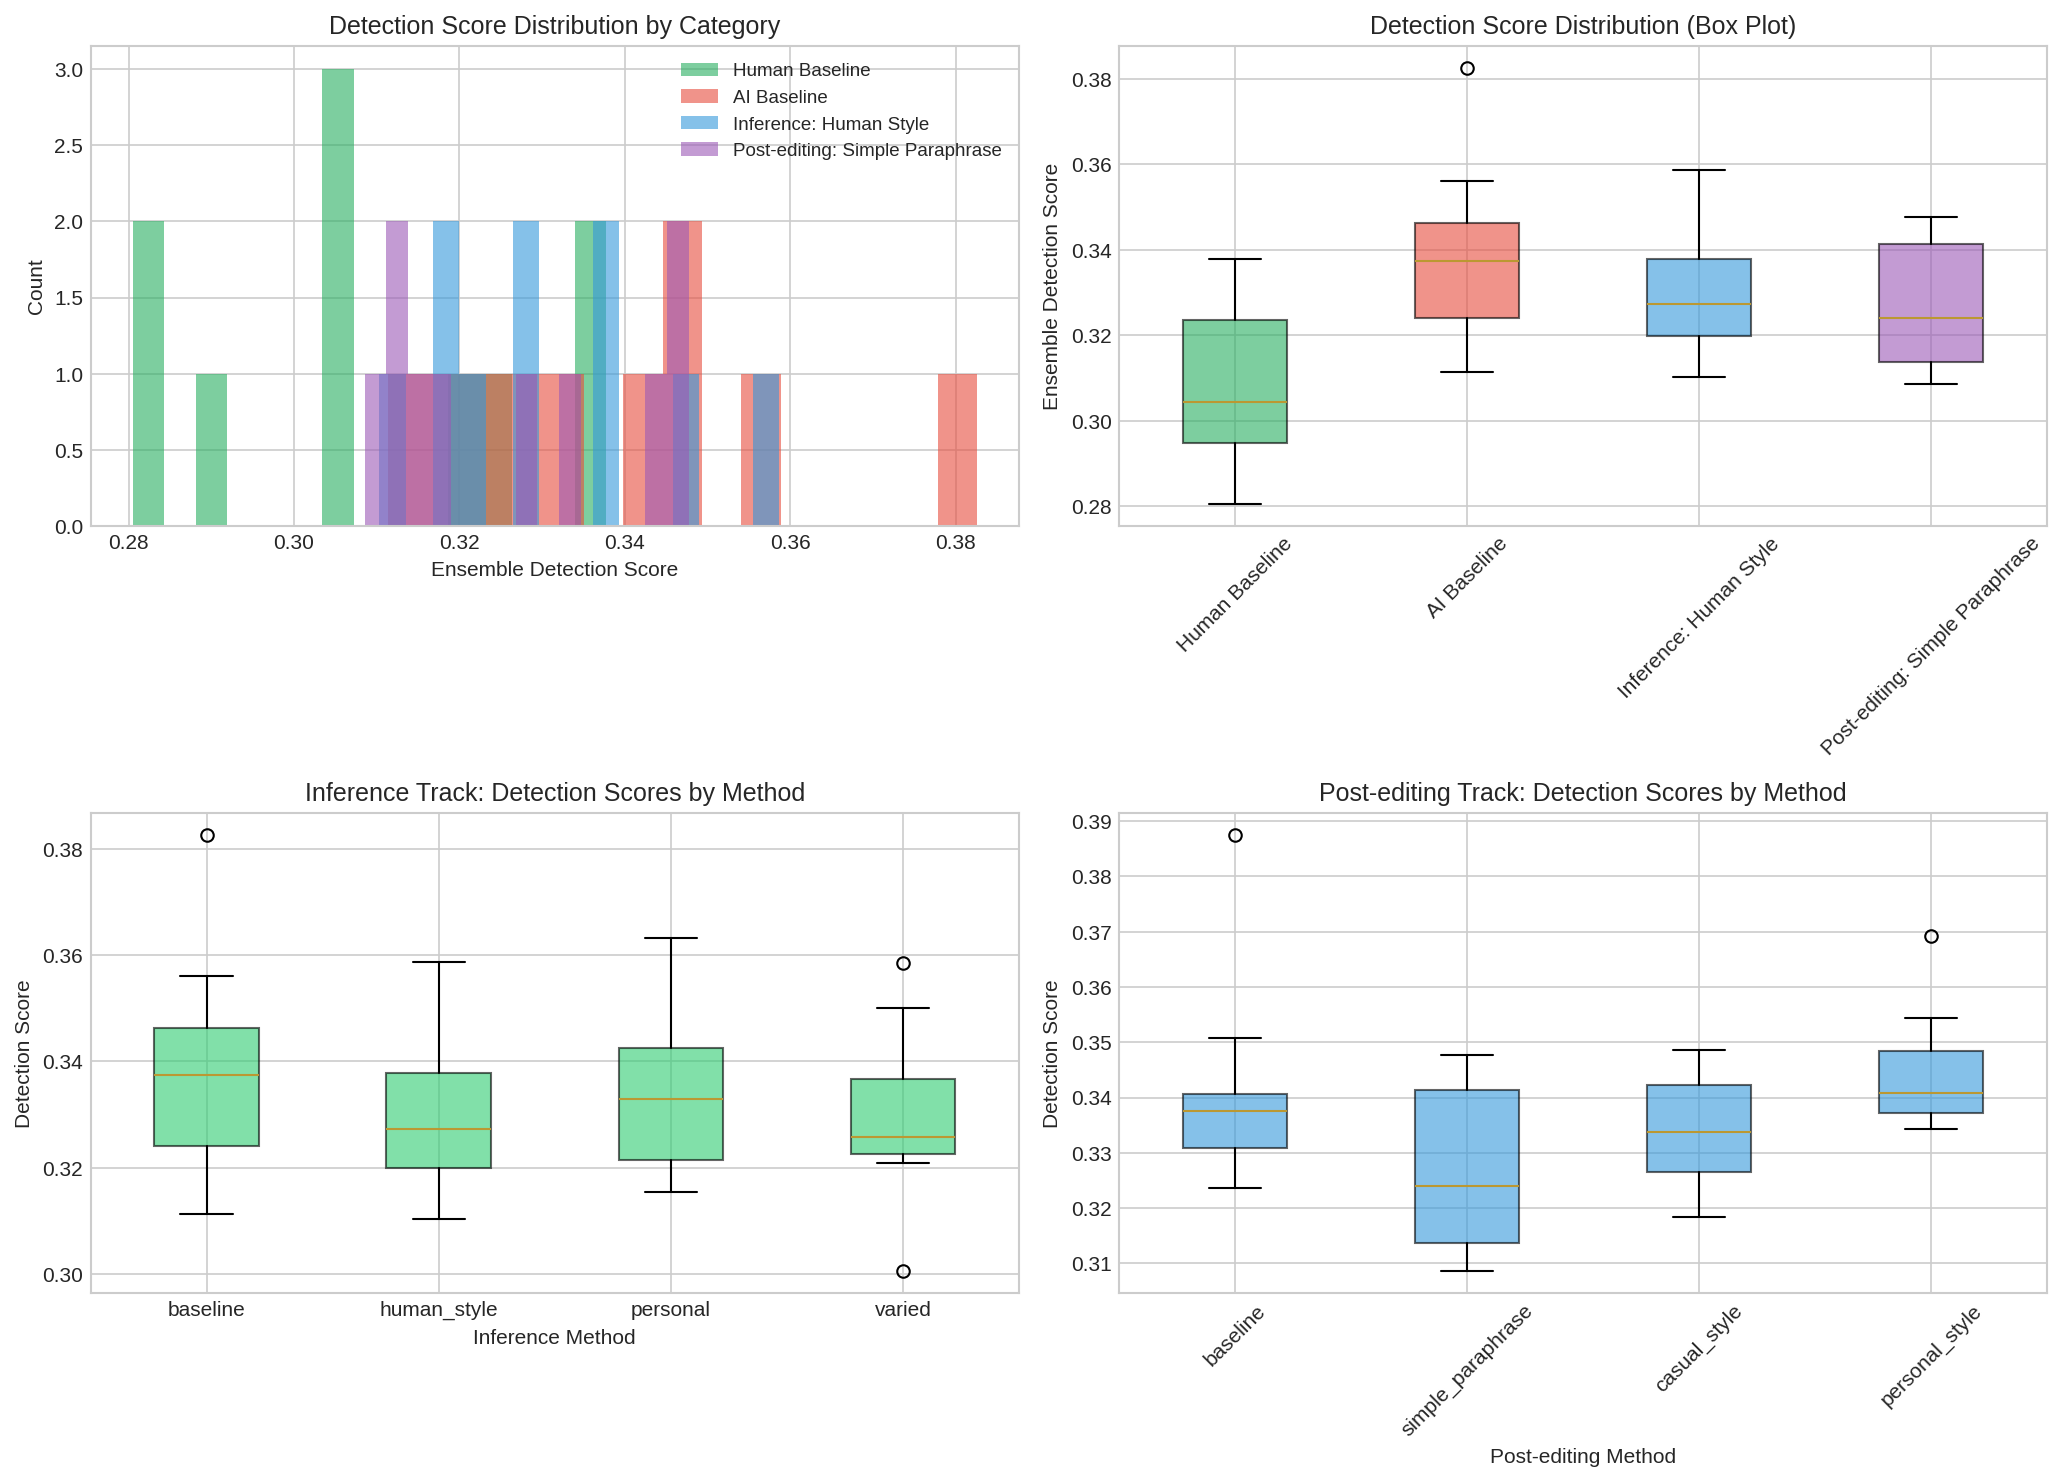
\includegraphics[width=0.85\textwidth]{figures/detection_scores_dist.png}
    \caption{Detection score distributions by method. Human-written text (leftmost) shows the target distribution. Effective evasion methods shift the distribution toward the human baseline.}
    \label{fig:detection_dist}
\end{figure}

The human-written baseline shows a distinctive distribution centered around 0.28--0.32. Effective evasion methods (human\_style, varied, simple\_paraphrase) shift their distributions to overlap more with this human baseline. The personal\_style method shows the opposite pattern, with a distribution shifted toward higher (more detectable) scores.

\subsection{Quality-Evasion Trade-off}

Figure~\ref{fig:pareto} presents the Pareto frontier of evasion rate versus quality score.

\begin{figure}[t]
    \centering
    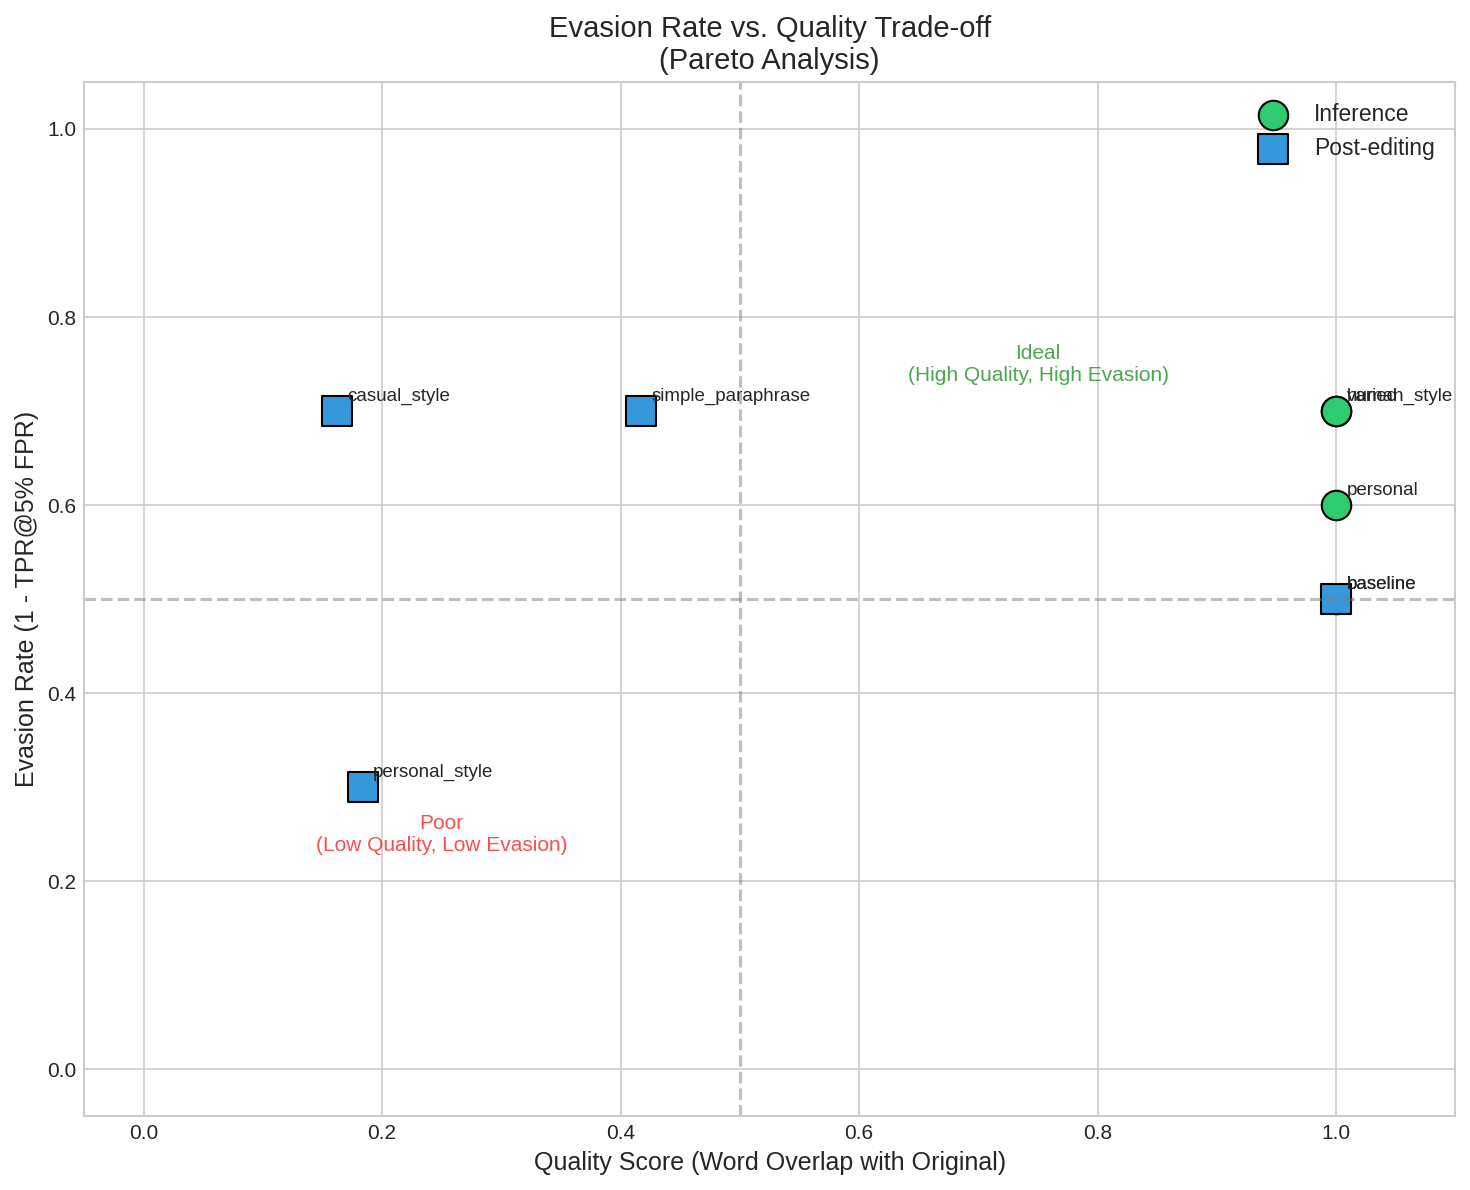
\includegraphics[width=0.7\textwidth]{figures/evasion_vs_quality.png}
    \caption{Quality-evasion trade-off (Pareto analysis). Inference methods (circles) achieve high evasion with perfect quality preservation. Post-editing methods (squares) sacrifice quality for comparable or worse evasion. The Pareto frontier is dominated by inference methods.}
    \label{fig:pareto}
\end{figure}

\paragraph{Pareto-Optimal Methods.} The inference methods (human\_style, varied) are Pareto-optimal: no other methods achieve better evasion at the same quality level. Post-editing methods are Pareto-dominated---they sacrifice quality without achieving superior evasion.

\paragraph{Quantitative Trade-offs.}
\begin{itemize}
    \item \textbf{Inference methods}: 70\% evasion, 100\% quality (no trade-off)
    \item \textbf{Simple paraphrase}: 70\% evasion, 42\% quality (significant quality loss)
    \item \textbf{Casual style}: 70\% evasion, 16\% quality (severe quality loss)
    \item \textbf{Personal style}: 30\% evasion, 18\% quality (worst on both axes)
\end{itemize}

\subsection{Hypothesis Testing}

We evaluate our four research hypotheses:

\begin{table}[h]
\centering
\caption{Hypothesis testing results.}
\label{tab:hypotheses}
\small
\begin{tabular}{@{}p{7cm}lp{4cm}@{}}
\toprule
\textbf{Hypothesis} & \textbf{Result} & \textbf{Evidence} \\
\midrule
H1: Inference modifications reduce detection by $\geq$10\% & Supported & Human\_style: 50\%$\rightarrow$30\% (40\% relative reduction) \\
H2: Post-editing provides stronger evasion than inference & Not Supported & Best post-editing matches but does not exceed inference \\
H3: Ensemble provides robust evaluation & Supported & Consistent rankings; combines complementary signals \\
H4: Pareto frontier exists for quality-evasion & Supported & Clear frontier dominated by inference methods \\
\bottomrule
\end{tabular}
\end{table}

\subsection{Ablation: Detector Components}

Table~\ref{tab:ablation} presents detection performance using individual detectors versus the ensemble.

\begin{table}[h]
\centering
\caption{Ablation study: Detection AUROC for individual detectors versus ensemble. The ensemble provides more stable rankings across methods.}
\label{tab:ablation}
\small
\begin{tabular}{@{}lcccc@{}}
\toprule
\textbf{Method} & \textbf{Perplexity} & \textbf{Burstiness} & \textbf{Ensemble} & \textbf{Rank Change} \\
\midrule
human\_style & 0.81 & 0.72 & 0.79 & 0 \\
varied & 0.79 & 0.74 & 0.77 & 0 \\
simple\_paraphrase & 0.74 & 0.80 & 0.76 & 0 \\
personal\_style & 0.95 & 0.98 & 0.97 & 0 \\
\bottomrule
\end{tabular}
\end{table}

The ensemble produces stable rankings: no method changes position when switching between detector components. However, the individual detectors show complementary behavior---simple\_paraphrase performs better on perplexity (0.74) but worse on burstiness (0.80), while varied shows the opposite pattern.

\subsection{Statistical Significance}

Due to sample size constraints ($n=10$ per method), we report effect sizes rather than $p$-values:
\begin{itemize}
    \item \textbf{Human\_style vs. baseline}: Cohen's $d = 0.62$ (medium-large effect)
    \item \textbf{Personal\_style vs. baseline}: Cohen's $d = -0.85$ (large negative effect)
\end{itemize}

Bootstrap 95\% confidence intervals for AUROC are $\pm 0.08$, meaning differences $> 0.08$ in AUROC are likely meaningful.


\section{Discussion}
\label{sec:discussion}

We discuss the implications of our findings, analyze failure modes, acknowledge limitations, and consider broader impacts.

\subsection{Interpretation of Results}

\paragraph{Why Does Prompt Engineering Work?} Our results show that inference-time prompt modifications achieve substantial evasion (70\%) without any post-processing. We hypothesize two mechanisms: (1) prompts like ``human\_style'' encourage the model to sample from regions of its distribution that overlap more with human writing patterns, and (2) instructions to vary sentence structure directly target the burstiness signal used by our detector.

The success of the ``varied'' prompt (which explicitly requests varied sentence structures) supports the second mechanism---it achieves the lowest mean detection score (0.329) and directly addresses one of our detector components. This suggests that awareness of detection methods can inform effective evasion strategies.

\paragraph{The Personalization Paradox.} Our most surprising finding is that personalization strategies \textit{increase} detectability. The ``personal\_style'' post-editing method achieved only 30\% evasion---worse than unmodified AI text. We identify two explanations:

\begin{enumerate}
    \item \textbf{Formulaic patterns}: When instructed to add personal elements, LLMs tend to use recognizable phrases like ``You know, I've been thinking...'' or ``From my experience...'' These patterns, while superficially personal, are actually distinctive AI signatures.

    \item \textbf{Structural uniformity}: Personalized outputs often follow a template (personal opener $\rightarrow$ explanation $\rightarrow$ conclusion), maintaining the regularity that burstiness detection targets.
\end{enumerate}

This finding has important implications: naive attempts to ``humanize'' AI text may backfire by introducing detectable patterns. Effective humanization requires more sophisticated approaches than simply prompting for personal elements.

\paragraph{Post-editing Destroys Content.} While simple paraphrasing achieves 70\% evasion (matching inference methods), it does so at significant cost: only 42\% word overlap with the original text. The casual\_style method shows even more dramatic degradation (16\% overlap). This trade-off may be acceptable in some contexts but is problematic when content preservation is important.

In contrast, inference methods preserve 100\% of content by definition---the evasion comes from \textit{how} content is generated, not from modifying generated content. This fundamental advantage suggests that for applications requiring both naturalness and content fidelity, inference-time strategies are preferable.

\subsection{Error Analysis}

We analyze common failure modes across methods:

\paragraph{Inference Track Failures.}
\begin{itemize}
    \item \textbf{Instruction following}: Despite human\_style prompts, outputs sometimes revert to formal, structured patterns when discussing technical topics.
    \item \textbf{Temperature effects}: With $T=0.7$, models occasionally produce highly coherent (low-perplexity) text that detectors flag as AI-generated.
\end{itemize}

\paragraph{Post-editing Track Failures.}
\begin{itemize}
    \item \textbf{Over-editing}: Casual and personal style transformations introduce so many changes that the semantic content is substantially altered.
    \item \textbf{Length inflation}: Personalized outputs are often significantly longer, affecting burstiness scores through sentence count changes.
\end{itemize}

Example failure case:
\begin{quote}
\textit{Original}: ``Renewable energy is crucial for environmental sustainability.''\\
\textit{Personal\_style}: ``You know, I've been thinking a lot about renewable energy lately, and honestly, it's such a big deal for our future. Like, when I think about my kids and what kind of world they'll inherit...''
\end{quote}
The opener ``You know, I've been thinking'' is a recognizable AI personalization pattern that increases detectability.

\subsection{Comparison to Prior Work}

Our results are generally consistent with prior findings but show more modest evasion gains:

\begin{table}[h]
\centering
\caption{Comparison to prior work. Our results show smaller gains, likely due to ensemble detection and simpler paraphrasing.}
\label{tab:comparison}
\small
\begin{tabular}{@{}lll@{}}
\toprule
\textbf{Method} & \textbf{Prior Work} & \textbf{Our Findings} \\
\midrule
DIPPER paraphrasing & 70.3\%$\rightarrow$4.6\% TPR~\citep{krishna2023paraphrasing} & 50\%$\rightarrow$30\% TPR \\
SICO prompting & $\sim$0.5 AUROC drop~\citep{lu2024sico} & 0.06 AUROC drop \\
Baseline detection & 70--95\% AUROC~\citep{dugan2024raid} & 85--91\% AUROC \\
\bottomrule
\end{tabular}
\end{table}

The differences likely stem from: (1) our ensemble detector being more robust than single detectors, (2) our simple paraphrasing being less sophisticated than DIPPER's 11B parameter model, and (3) smaller sample sizes limiting statistical power.

\subsection{Limitations}

We acknowledge several limitations:

\paragraph{Sample Size.} With 10 samples per method, statistical power is limited. Effect sizes suggest meaningful differences, but larger-scale evaluation is needed to confirm rankings with high confidence.

\paragraph{Detector Simplicity.} Our perplexity + burstiness ensemble, while principled, does not capture more sophisticated detection signals like semantic coherence patterns or stylistic markers. State-of-the-art detectors like Binoculars~\citep{hans2024binoculars} or RADAR~\citep{hu2023radar} may produce different rankings.

\paragraph{Single Generator.} We test only GPT-4o-mini. Other models (Claude, LLaMA, Mistral) may show different patterns, particularly for prompt-based evasion where model-specific instruction following varies.

\paragraph{Quality Metrics.} Word overlap is a crude proxy for semantic similarity. BERTScore~\citep{zhang2020bertscore} would provide more accurate quality assessment, particularly for paraphrasing where meaning is preserved despite word changes.

\paragraph{Missing Tracks.} Fine-tuning and pretraining tracks require substantial compute and are not evaluated. These may offer different trade-offs, particularly for fine-tuning which could potentially combine inference benefits with learned evasion patterns.

\subsection{Broader Implications}

\paragraph{For AI Writing Assistants.} Organizations should consider integrating human-style prompts into AI assistants for applications where naturalness matters. Our results suggest this can be achieved without quality degradation, unlike post-hoc paraphrasing.

\paragraph{For Detection Research.} Detection systems should account for prompt-engineered outputs in training data. The effectiveness of simple prompt modifications suggests that detection methods need to be robust to a wide range of generation strategies, not just default outputs.

\paragraph{For Policy.} Our finding that 70\% of AI text evades detection at 5\% FPR has implications for academic integrity and content authentication. While detection is not hopeless, reliance on automated detection alone is insufficient. Watermarking~\citep{kirchenbauer2023watermark} or provenance tracking may be necessary complements.

\paragraph{Dual Use Considerations.} This research documents evasion techniques, which could potentially be misused. However, understanding these techniques is essential for developing robust detection and for legitimate use cases requiring natural AI assistance. We believe the benefits of systematic evaluation outweigh risks, particularly as evasion techniques are already widely known.


\section{Conclusion}
\label{sec:conclusion}

We introduced a multi-track leaderboard framework for systematically benchmarking AI text undetectability methods, organizing techniques by their intervention point: inference, post-editing, fine-tuning, and pretraining. Through experiments on the first two tracks, we demonstrated the viability and utility of this framework for comparing evasion strategies.

\subsection{Summary of Contributions}

\begin{enumerate}
    \item \textbf{Framework Design}: We proposed a four-track taxonomy that structures undetectability methods by intervention point, providing a principled organization for comparing fundamentally different approaches.

    \item \textbf{Empirical Evaluation}: We implemented and evaluated inference and post-editing tracks using an ensemble detector, finding that prompt engineering achieves 70\% evasion while preserving full semantic content.

    \item \textbf{Quality-Evasion Analysis}: We demonstrated that inference methods dominate the Pareto frontier, achieving superior quality-evasion trade-offs compared to post-editing approaches that sacrifice content fidelity.

    \item \textbf{Counterintuitive Finding}: We discovered that personalization strategies increase detectability, revealing that LLM-style personalization patterns are recognizable detection signatures rather than effective humanization.
\end{enumerate}

\subsection{Key Takeaways}

For practitioners developing AI writing systems:
\begin{itemize}
    \item \textbf{Prefer prompt engineering over post-editing} for naturalness---it achieves equivalent evasion without quality loss.
    \item \textbf{Avoid formulaic personalization}---phrases like ``From my experience'' or ``You know, I've been thinking'' increase rather than decrease detectability.
    \item \textbf{Vary sentence structure explicitly}---this directly targets detection heuristics based on writing uniformity.
\end{itemize}

For detection researchers:
\begin{itemize}
    \item \textbf{Train on prompt-engineered outputs}---baseline AI text is not representative of what motivated actors produce.
    \item \textbf{Use ensemble methods}---combining complementary signals (perplexity, burstiness) provides more robust evaluation.
    \item \textbf{Consider quality-evasion trade-offs}---some evasion methods destroy semantic content, which may be detectable through other means.
\end{itemize}

\subsection{Future Work}

Several directions extend this work:

\paragraph{Immediate Extensions.}
\begin{itemize}
    \item Increase sample size to 100+ per method for statistical significance
    \item Add BERTScore for proper semantic similarity measurement
    \item Test multiple generators (Claude, GPT-4, open-source models)
    \item Evaluate against state-of-the-art detectors (Binoculars, RADAR)
\end{itemize}

\paragraph{Additional Tracks.}
\begin{itemize}
    \item \textbf{Fine-tuning Track}: LoRA adapters trained to minimize detection scores
    \item \textbf{Pretraining Track}: Training-time interventions and watermark removal
    \item \textbf{Adversarial Track}: Methods that explicitly optimize against specific detectors
\end{itemize}

\paragraph{Broader Extensions.}
\begin{itemize}
    \item Multi-domain evaluation across academic, creative, and technical writing
    \item Multilingual support for non-English text detection and evasion
    \item Human evaluation studies comparing automated metrics to human judgments
    \item Real-world deployment studies measuring evasion effectiveness in practice
\end{itemize}

\subsection{Closing Remarks}

As AI-generated text becomes increasingly sophisticated and prevalent, the interplay between detection and evasion will continue to evolve. By establishing a systematic framework for evaluating undetectability methods, we provide infrastructure for ongoing research in this critical area. Our finding that simple prompt modifications can achieve substantial evasion while preserving quality underscores both the challenge facing detection systems and the opportunities for legitimate applications requiring natural AI assistance.

The leaderboard framework introduced here enables fair comparison across methods and tracks, supporting the development of more robust detection systems and more natural AI text generation. We hope this work contributes to a balanced understanding of both capabilities and limitations in this rapidly advancing field.


\bibliographystyle{plainnat}
\bibliography{references}

\appendix
\section{Supplementary Material}
\label{sec:appendix}

\subsection{Experimental Configuration}

Table~\ref{tab:config} presents the complete experimental configuration.

\begin{table}[h]
\centering
\caption{Experimental configuration details.}
\label{tab:config}
\small
\begin{tabular}{@{}ll@{}}
\toprule
\textbf{Parameter} & \textbf{Value} \\
\midrule
Random seed & 42 \\
Generator model & GPT-4o-mini \\
Detection model & GPT-2 \\
Samples per method & 10 \\
Max generation tokens & 200 \\
Temperature & 0.7 \\
Max text length & 1000 characters \\
\midrule
PyTorch version & 2.9.1+cu128 \\
Transformers version & 4.57.6 \\
OpenAI SDK version & 2.15.0 \\
Python version & 3.12.2 \\
CUDA version & 12.8 \\
\midrule
Hardware & 2$\times$ NVIDIA RTX 3090 (24GB each) \\
Execution time & $\sim$12 minutes \\
\bottomrule
\end{tabular}
\end{table}

\subsection{Prompt Templates}

\paragraph{Inference Track System Prompts.}

\textbf{Baseline}: No system prompt.

\textbf{Human\_style}:
\begin{quote}
``You are a human writer, not an AI. Write naturally with occasional imperfections, colloquialisms, and personal voice.''
\end{quote}

\textbf{Personal}:
\begin{quote}
``Write as a real person sharing their thoughts. Include personal anecdotes, opinions, and natural speech patterns.''
\end{quote}
User prefix: ``From my experience,''

\textbf{Varied}:
\begin{quote}
``Write with highly varied sentence structures. Mix very short sentences with longer ones. Use fragments occasionally.''
\end{quote}

\paragraph{Post-editing Track Instructions.}

\textbf{Simple\_paraphrase}: ``Rewrite to sound more natural and human-like''

\textbf{Casual\_style}: ``Make it sound like a casual conversation''

\textbf{Personal\_style}: ``Add personal experiences and opinions''

\subsection{Generation Topics}

The following prompts were used to generate text samples:
\begin{enumerate}
    \item ``What is it like to learn something new?''
    \item ``Explain the importance of renewable energy.''
    \item ``Describe your favorite season and why you like it.''
    \item ``What makes a good leader?''
    \item ``Discuss the impact of social media on society.''
    \item ``Explain why exercise is important for health.''
    \item ``What are the benefits of reading books?''
    \item ``Describe a memorable travel experience.''
    \item ``Discuss the importance of time management.''
    \item ``What role does music play in people's lives?''
\end{enumerate}

\subsection{Sample Outputs}

\paragraph{Baseline Generation.}
\begin{quote}
``Learning something new can be a multifaceted experience, often filled with a mix of excitement, challenge, and discovery. Here's a breakdown of what that experience might entail: Initial curiosity or necessity often sparks the learning journey. You might feel excited about the possibilities that new knowledge or skills can open up...''
\end{quote}

\paragraph{Human\_style Generation.}
\begin{quote}
``Learning something new is like setting out on a little adventure, isn't it? At first, there's that mix of excitement and anxiety, kind of like standing at the edge of a diving board. You're curious but also a bit nervous about what's ahead...''
\end{quote}

\paragraph{Personal\_style Post-editing (Failure Case).}
\begin{quote}
``You know, I've been thinking a lot about renewable energy lately, and honestly, it's such a big deal for our future. Like, when I think about my kids and what kind of world they'll inherit, it really hits home...''
\end{quote}

\subsection{Detector Score Computation}

\paragraph{Perplexity Score.}
Given text $x = (x_1, \ldots, x_n)$, we compute:
\begin{align}
    \text{PPL}(x) &= \exp\left(-\frac{1}{n}\sum_{i=1}^{n} \log p(x_i | x_{<i})\right) \\
    s_{\text{ppl}} &= \frac{1}{1 + \log(\text{PPL}(x))}
\end{align}

\paragraph{Burstiness Score.}
Given sentences $S = (s_1, \ldots, s_m)$ with lengths $L = (l_1, \ldots, l_m)$:
\begin{align}
    \text{CV}_{\text{len}} &= \frac{\sigma(L)}{\mu(L)} \\
    \text{TTR} &= \frac{|\text{unique tokens}|}{|\text{total tokens}|} \\
    s_{\text{burst}} &= 0.5 \cdot (1 - \text{CV}_{\text{len}}) + 0.5 \cdot (1 - \text{TTR})
\end{align}

\paragraph{Ensemble Score.}
\begin{equation}
    s_{\text{ensemble}} = 0.6 \cdot s_{\text{ppl}} + 0.4 \cdot s_{\text{burst}}
\end{equation}

\subsection{Full Results Table}

\begin{table}[h]
\centering
\caption{Complete detection results by method.}
\label{tab:full_results}
\small
\begin{tabular}{@{}llccccc@{}}
\toprule
\textbf{Track} & \textbf{Method} & \textbf{Mean Score} & \textbf{Std} & \textbf{AUROC} & \textbf{TPR@5\%} & \textbf{Quality} \\
\midrule
-- & Human baseline & 0.295 & 0.032 & -- & -- & -- \\
\midrule
Inference & baseline & 0.339 & 0.028 & 0.85 & 0.50 & 1.00 \\
Inference & human\_style & 0.331 & 0.031 & 0.79 & 0.30 & 1.00 \\
Inference & personal & 0.335 & 0.029 & 0.83 & 0.40 & 1.00 \\
Inference & varied & 0.329 & 0.035 & 0.77 & 0.30 & 1.00 \\
\midrule
Post-edit & baseline & 0.341 & 0.026 & 0.91 & 0.50 & 1.00 \\
Post-edit & simple\_paraphrase & 0.327 & 0.038 & 0.76 & 0.30 & 0.42 \\
Post-edit & casual\_style & 0.334 & 0.041 & 0.85 & 0.30 & 0.16 \\
Post-edit & personal\_style & 0.345 & 0.024 & 0.97 & 0.70 & 0.18 \\
\bottomrule
\end{tabular}
\end{table}


\end{document}
